\documentclass[tikz,border=2pt]{standalone}
\usepackage{amsmath,amssymb}
\usepackage{tikz}
\usetikzlibrary{arrows.meta}

\begin{document}
% A vector of R^2 is an ordered pair of coordinates, pictured as an arrow; translating the
% arrow does not change the vector.
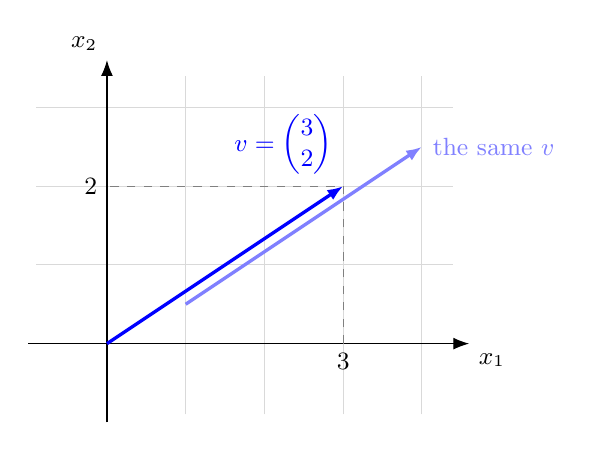
\begin{tikzpicture}[every node/.style={font=\small}, >={Latex[length=2mm]}]
	\draw[gray!30, step=1] (-0.9,-0.9) grid (4.4,3.4);
	\draw[->] (-1,0) -- (4.6,0) node[below right] {$x_1$};
	\draw[->] (0,-1) -- (0,3.6) node[above left] {$x_2$};
	\draw[dashed, gray] (3,0) -- (3,2) -- (0,2);
	\draw[->, blue, very thick] (0,0) -- (3,2) node[above left] {$v=\begin{pmatrix}3\\2\end{pmatrix}$};
	\node[below, font=\small] at (3,0) {$3$};
	\node[left, font=\small] at (0,2) {$2$};
	\draw[->, blue!50, very thick] (1,0.5) -- (4,2.5) node[right, font=\small] {the same $v$};
\end{tikzpicture}
\end{document}
